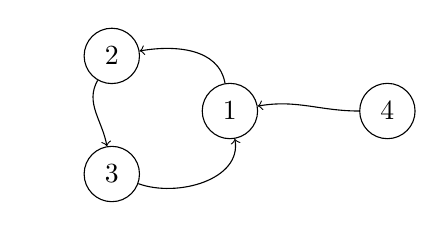
\begin{tikzpicture}
\tikzstyle{every node}=[draw,circle,fill=white,minimum size=20pt,
inner sep=0pt]

\draw (-1.5,0)  node (2) [label=left:$$] {2};
\draw (-1.5 ,-1.5)  node (3) [label=left:$$] {3};
\draw (0,-0.7)  node (1) [label=left:$$] {1};
\draw [->] (2) to  [out = 240, in = 100] (3);
\draw [->] (1)to  [out = 100, in = 10](2);
\draw [->] (3)to  [out = 340, in = 280](1);
\draw (2,-0.7)  node (4) [label=left:$$] {4};
\draw [->] (4)to  [out = 180, in = 10](1);
\end{tikzpicture}